\documentclass[a4paper,12pt]{article} %style de document
\usepackage{graphicx, epsfig,subfigure}
\usepackage[french]{babel}
\usepackage{fancyhdr}
\usepackage{titlesec}
\usepackage{graphicx}
\usepackage{hyperref}
\pagestyle{fancy}
\fancyhead[R]{}
\fancyfoot[L]{Pré-rapport projet POO}
\fancyfoot[R]{Annéé 2022-2023}


\author{Mis en page par \\
   KEFI Elias, \\
   L1 info,\\
   Groupe 2,\\}
\begin{document}
\title{Pré-rapport de KEFI Elias, LAMBERTZ Nathan et GENESTIER Théo}

\titleformat{\section}
{\centering\large\bfseries}
{\thesection}
{1em}
{}

\titleformat{\subsection}
{\centering\normalsize\bfseries}
{\thesubsection}
{1em}
{}


\maketitle

\includegraphics[scale=1]{./Images/logoUnicaen.png}


\newpage
\tableofcontents
\newpage

\section{Introduction}
Suite au TP Fil rouge, et des créations des classe Elements, Animal et de toutes celles faites en TP. Voici les modifications que nous avons pensé intéressantes à apporter pour notre projet:

\section{Fonctionnalités prévues}

Nous allons vous présenter les quelques idées de fonctionnalités que nous aimerions ajoutées:
\newline
\begin{itemize}
\item[•]La rencontre de deux animaux de même espèce et de sexe différents crée un bébé de cette espèce. Le bébé sera représenté par un animal de '0 an(s)' et non par une autre classe.  
\newline
\item[•]Quand deux lapins de sexe différents se rencontrent, ils donnent naissance à un nombre de lapereaux aléatoire entre 1 et 12.
\newline
\item[•]Quand deux êtres vivants se rencontrent, un évènement aléatoire se lancera pour celui qui a la barre de vie la plus faible. Le résultat sera soit 0 soit 1. Si 0 tombe, alors il meurt. Si c'est 1, un évènement naturel (séisme, tornade, éruption...) se déclenchera parmi une liste et sauvera l'animal. Par exemple si une vache et un dragon se rencontrent, l'évènement qui donne 0 ou 1 se lance. Si c'est 0, la vache meurt. Si c'est 1, la vache est sauvée par un séisme.
\newline
\item[•]Ajout de différents êtres vivants en plus de ceux faits en TP tel que des serpents, des hommes et des chevaliers.
\newline
\item[•]Un système de tours dans lequel chaque être vivant à une distance de déplacement possible à chaque tour. Par exemple, une souris peu se déplacer de 3 cases et un dragon de 10 cases. Les déplacement ne seront pas totalement aléatoire, par exemple si la souris est proche d'un dragon. Il y a 70\% de chance que la souris s'en aille.
\newline
\item[•]Quand deux ovipares de même espèce et de sexe différents se rencontrent, ils donnent naissance à 5 œufs qui écloront après X tours. 
\newline
\item[•]Et la meilleure idée de ce projet, les vaches meugleront toutes les 10 secondes avec une petite bulle ou il sera écrit "MOO!".

\end{itemize}

\section{Interface graphique}
\subsection{Map}
\begin{minipage}{0.95\textwidth}
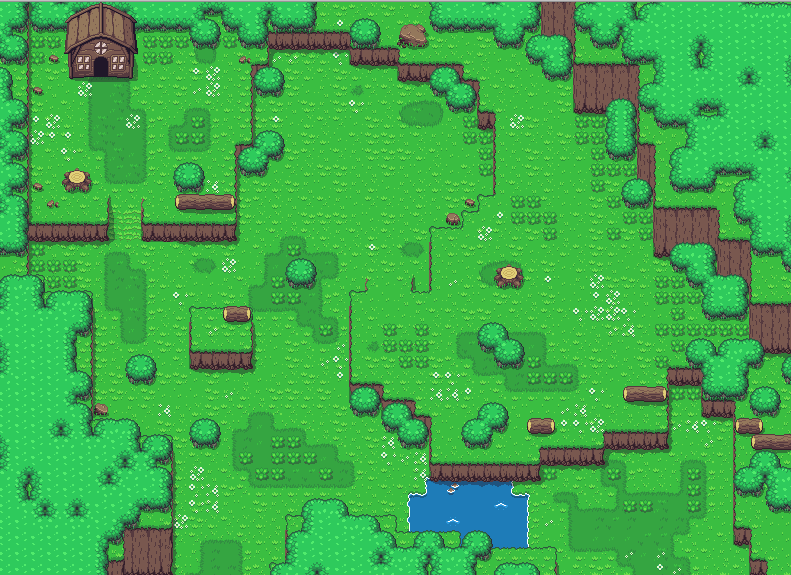
\includegraphics[width=\linewidth]{./Images/map.png}
\end{minipage}
\newline
\newline
Voici la map sur laquelle les êtres vivants vont se déplacer, ils se déplaceront donc avec le système de cases expliqué plus tôt. La taille d'une case correspondra environ a la taille d'une plante. Avec ce système, on pourra empêcher aux êtres vivants de traverser les murs, les arbres ou la maison. Certains animaux ne pourront pas aller dans l'eau comme les souris par exemple.

\subsection{Déplacement des sprites}
Les différents êtres vivants auront un sprite associé. Le sprite ne regardera que dans deux directions: à droite quand il vas vers une case à droite ou en haut, à gauche quand il vas à gauche ou en bas.
\newpage
\begin{center}
Par exemple (pour le dragon):

\includegraphics[scale=0.6]{./Images/dragon.jpeg}

Ce sprite sera actif quand le dragon se déplacera vers la gauche ou vers le bas.

\reflectbox{\includegraphics[scale=0.6]{./Images/dragon.jpeg}}
\item
Ce sprite sera actif quand le dragon se déplacera vers la droite ou vers le haut.

\end{center}






\section{Diagramme de GANTT}
\begin{minipage}{1.1\textwidth}
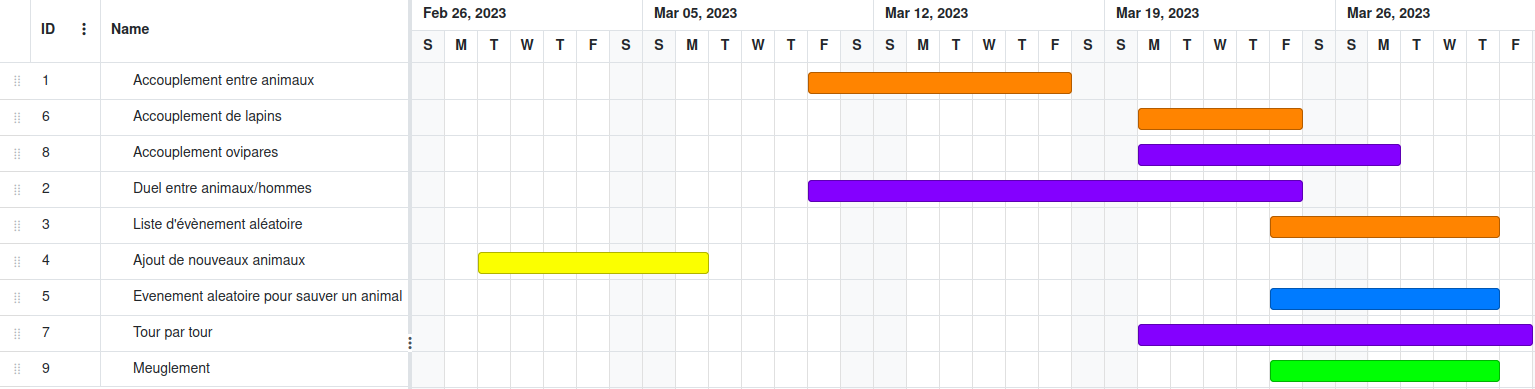
\includegraphics[width=\linewidth]{./Images/gantt.png}
\end{minipage}



\subsection{Répartition des tâches}


\begin{itemize}
\item[•] Orange : Nathan et Théo.
\item[•] Violet : Elias, Nathan et Théo
\item[•] Bleu : Théo
\item[•] Jaune : Elias et Nathan
\item[•] Vert : Elias
\end{itemize}

\subsection{Précision sur le Gantt}


Le diagramme de Gantt a été fait en fonction des fonctionnalités que nous avions prévues de faire. En revanche qui s'en occupera et combien de temps cela prendra, ce ne sont que de vagues approximations car nous ne savons pas quels problèmes nous allons rencontrés.
\newline

\section{Diagramme de classes UML}


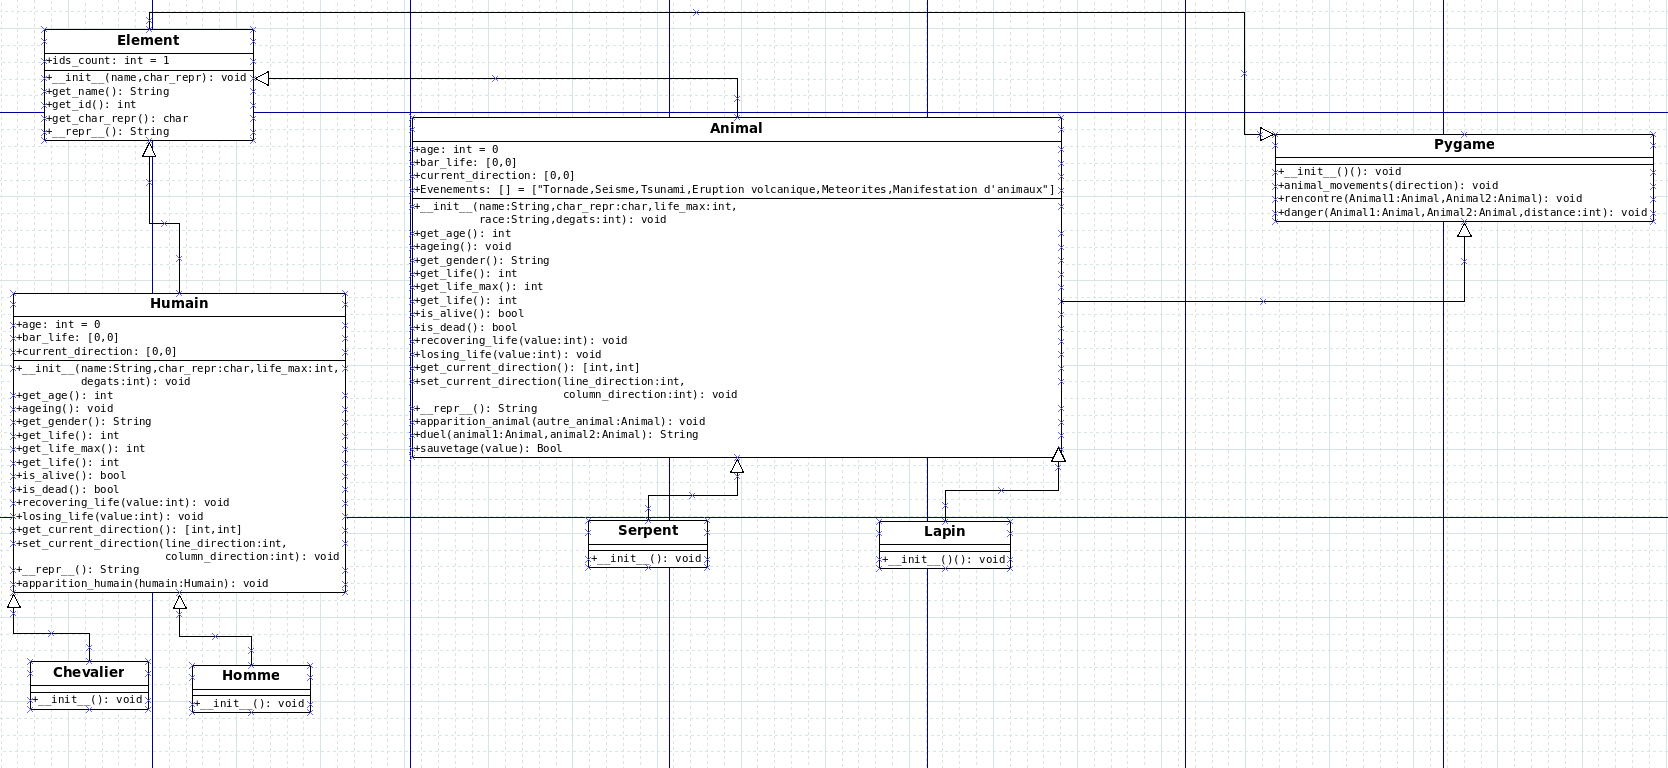
\includegraphics[scale=0.25]{./Images/uml.png}

Voici le diagramme de classe de notre projet, il décrit les différentes relations entre les classes et quelles méthodes appartiennent a quelles classes. 

\section{Chef de projet}


Nous avons choisi KEFI Elias pour être le responsable de notre projet. Il devra donc gérer l'avancée du projet, à chaque début de cours. Et donc mettre à jour le diagramme de gantt pour avoir le temps de faire toutes les tâches prévues.
\newline
De plus, il se chargera de la bonne avancée du projet ainsi que de l'avancement des tâches de chacun.



\end{document}